\chapter{Técnicas y herramientas}
\label{chap:tecnicas_herramientas}

En este capítulo se describen en detalle las principales tecnologías, lenguajes de programación y herramientas que han constituido la base para el desarrollo de este Trabajo de Fin de Grado. El objetivo de esta sección es presentar cada componente de forma objetiva, explicando su función, características y arquitectura principal.

\section{Herramientas de Desarrollo y Gestión}
\label{sec:herramientas_desarrollo}

\subsection{Python}
Python es un lenguaje de programación de alto nivel, interpretado y multiparadigma, cuya filosofía de diseño enfatiza la legibilidad del código \cite{python_software_foundation}. Es mantenido por la Python Software Foundation y cuenta con una vasta biblioteca estándar y un ecosistema de librerías de terceros que lo han convertido en un estándar de facto en el desarrollo de aplicaciones, la ciencia de datos y el \textit{machine learning}.

\subsection{Jira y Metodología Ágil}
Jira es una herramienta de software desarrollada por Atlassian para el seguimiento de incidencias y la gestión de proyectos \cite{atlassian_jira}. Está diseñada para dar soporte a metodologías de desarrollo ágil como Scrum, que se basa en la organización del trabajo en iteraciones cortas denominadas Sprints. Jira facilita la gestión de un \textit{backlog} de tareas, la planificación de Sprints y la visualización del flujo de trabajo mediante tableros Kanban.

\begin{figure}[H]
    \centering
    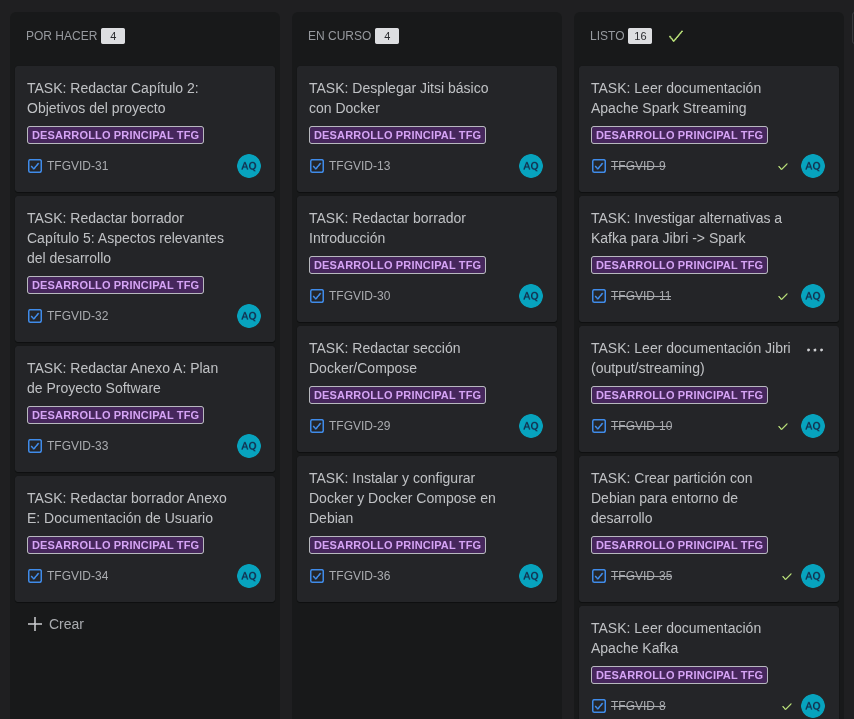
\includegraphics[width=\textwidth]{img/jira.png}
    \caption{Ejemplo del tablero Kanban utilizado en Jira para el seguimiento de las tareas del Sprint.}
    \label{fig:tablero_jira}
\end{figure}

\begin{figure}[H]
    \centering
    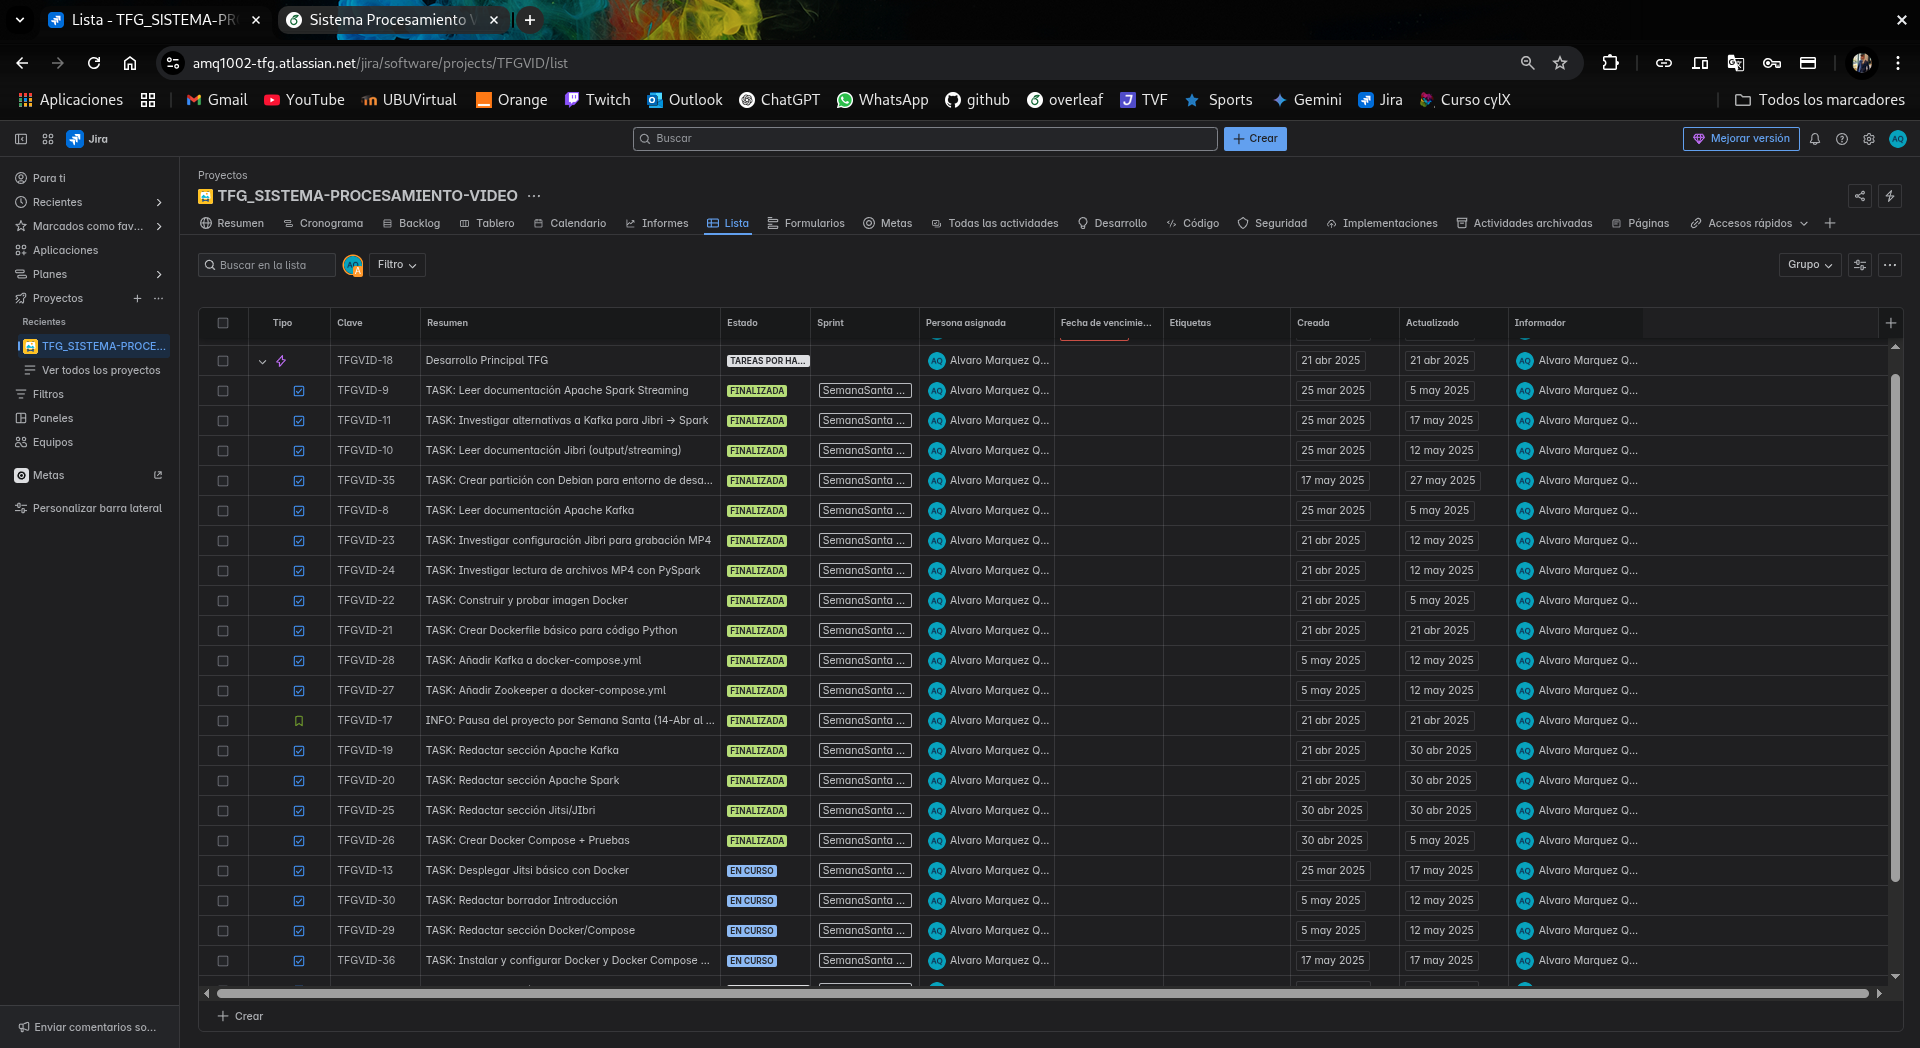
\includegraphics[width=\textwidth]{img/jira (2).png}
    \caption{Ejemplo del tablero Kanban utilizado en Jira para el seguimiento de las tareas del Sprint.}
    \label{fig: Jira ejemplo doc}
\end{figure}

\section{Infraestructura y Pipeline de Datos}
\label{sec:herramientas_infraestructura}
El núcleo del proyecto reside en la infraestructura diseñada para capturar, transportar y procesar los datos de vídeo.

\subsection{Contenerización con Docker y Docker Compose}
Docker es una plataforma de código abierto que automatiza el despliegue de aplicaciones dentro de contenedores \cite{docker_docs}. Un contenedor es una unidad de software estándar, ligera y ejecutable que incluye todo lo necesario para que una aplicación se ejecute: código, \textit{runtime}, herramientas del sistema y librerías. A diferencia de las máquinas virtuales, los contenedores comparten el kernel del sistema operativo anfitrión, lo que los hace mucho más eficientes en el uso de recursos. La gestión de contenedores se realiza a través de un \textbf{Dockerfile}, un fichero de texto que contiene las instrucciones para construir una imagen de contenedor.

Para la orquestación de los múltiples contenedores de este proyecto, se utiliza \textbf{Docker Compose}. Esta herramienta permite definir y gestionar aplicaciones multi-contenedor a través de un único archivo de configuración en formato YAML (\texttt{docker-compose.yml}). En este fichero se definen los diferentes servicios que componen la aplicación, sus imágenes, las redes que los conectan, los volúmenes de datos para la persistencia y las dependencias de arranque entre ellos.

\subsection{Plataforma de Videoconferencia: Jitsi}
Jitsi es una colección de proyectos de software libre para construir soluciones de videoconferencia seguras y escalables \cite{JitsiJibriDocs}. Su arquitectura es distribuida y se compone de varios microservicios que trabajan de forma coordinada:
\begin{itemize}
    \item \textbf{Jitsi Meet:} Es la aplicación cliente, una interfaz web basada en JavaScript y WebRTC que se ejecuta en el navegador del usuario y le permite participar en las conferencias.
    \item \textbf{Jitsi Videobridge (JVB):} Es el componente central. Funciona como una Unidad de Reenvío Selectivo (SFU), lo que significa que recibe los flujos de vídeo de cada participante y los reenvía de forma selectiva al resto, sin necesidad de decodificarlos y mezclarlos. Esta arquitectura es clave para la eficiencia y escalabilidad del sistema.
    \item \textbf{Prosody:} Es el servidor \textit{XMPP} que gestiona la señalización en las conferencias: quién entra o sale de una sala, el estado de los participantes, los mensajes de chat, etc.
    \item \textbf{Jicofo (Jitsi Conference Focus):} Actúa como el "director de orquesta" de las conferencias. Es el componente que gestiona las sesiones, invita a los nuevos participantes (incluido Jibri) a la conferencia y asigna los flujos de vídeo al Jitsi Videobridge.
    \item \textbf{Jibri (Jitsi Broadcasting Infrastructure):} Es el componente utilizado en este TFG para la captura de datos. Jibri es un servicio que se une a una conferencia como un participante silencioso, lanza una instancia de un navegador Chrome en un servidor virtual (\textit{headless}) y utiliza FFmpeg para capturar y grabar la vista compuesta de la conferencia en un archivo de vídeo estándar (formato MP4).
\end{itemize}

\begin{figure}[H]
    \centering
    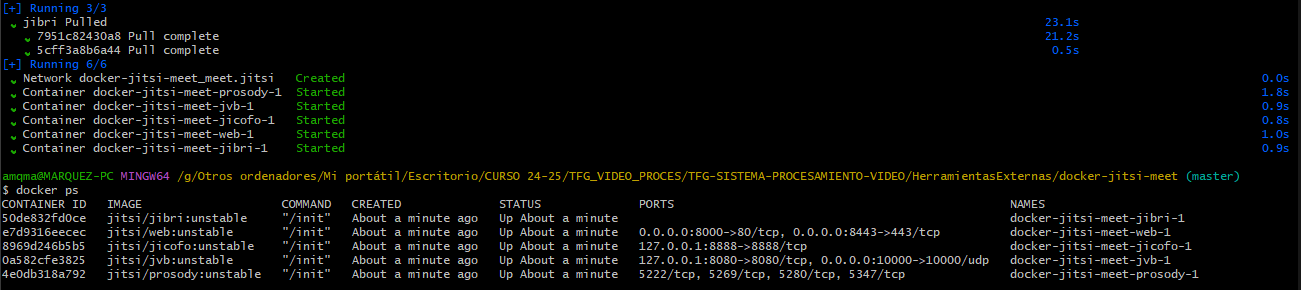
\includegraphics[width=\textwidth]{img/jitsimeet.png}
    \caption{Contenedores levantados para videoconferencia Jitsi.}
    \label{fig:Jitsi meet contenedores}
\end{figure}

\subsection{Plataformas de Big Data: Kafka y Spark}
\subsubsection{Apache Kafka: Un Log de Transacciones Distribuido}
Apache Kafka es una plataforma distribuida de código abierto para la transmisión de eventos (\textit{event streaming}) \cite{KafkaWebDoc}. Aunque a menudo se utiliza como un sistema de mensajería publicar-suscribir, su arquitectura fundamental es la de un \textbf{log de transacciones distribuido, particionado y replicado}. Los conceptos clave de su arquitectura son:
\begin{itemize}
    \item \textbf{Brokers y Clúster:} Kafka se ejecuta como un clúster de uno o más servidores, denominados \textit{brokers}. Estos brokers gestionan el almacenamiento y la atención a las peticiones de los clientes.
    \item \textbf{Topics y Particiones:} Los flujos de eventos se organizan en categorías llamadas \textit{topics}. Para permitir el paralelismo y la escalabilidad, cada topic se divide en una o más \textit{particiones}. Cada partición es un log ordenado e inmutable al que solo se pueden añadir nuevos registros.
    \item \textbf{Productores y Consumidores:} Las aplicaciones que escriben datos en los topics de Kafka se denominan \textit{Productores}. Las que leen los datos son los \textit{Consumidores}, que se organizan en grupos para procesar los datos de forma paralela.
    \item \textbf{Modo KRaft (sin Zookeeper):} Las versiones modernas de Kafka, como la utilizada en este proyecto, pueden operar en modo KRaft (Kafka Raft). En este modo, Kafka utiliza un protocolo de consenso interno para gestionar los metadatos del clúster, eliminando la necesidad de un sistema de coordinación externo como Apache Zookeeper y simplificando así significativamente la arquitectura de despliegue.
\end{itemize}

\begin{figure}[H]
    \centering
    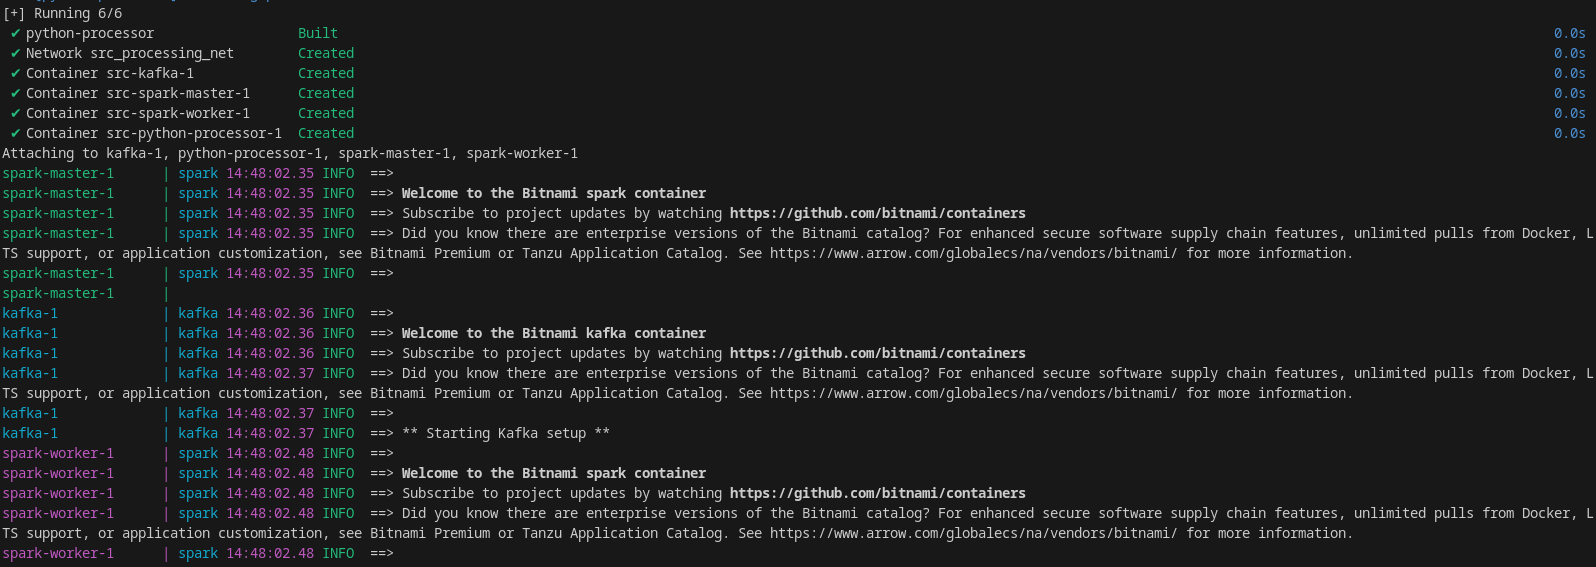
\includegraphics[width=\textwidth]{img/montarsparkkafka.png}
    \caption{Contenedores de Spark y Kafka iniciandose}
    \label{fig:MontajeSparkKafka}
\end{figure}

\subsubsection{Apache Spark: Un Motor de Computación Distribuida}
Apache Spark es un motor de análisis unificado para el procesamiento de datos a gran escala \cite{SparkWebDoc}. Su principal característica es su capacidad para realizar computación distribuida en memoria, lo que le permite alcanzar un alto rendimiento. Su arquitectura se compone de:
\begin{itemize}
    \item \textbf{Driver y Executors:} Una aplicación Spark consiste en un proceso \textit{driver} que coordina la ejecución y múltiples procesos \textit{executor} que se ejecutan en los nodos de un clúster. El driver analiza el código, planifica las tareas y las envía a los \textit{executors} para que las ejecuten en paralelo sobre los datos.
    \item \textbf{DataFrames y el Optimizador Catalyst:} La API principal de Spark es el DataFrame, una abstracción de datos distribuidos organizados en columnas con nombre. Cuando se ejecutan operaciones sobre un \textit{DataFrame}, el optimizador de Spark, llamado \textbf{Catalyst}, traduce estas operaciones a un plan lógico, lo optimiza y genera un plan físico de ejecución que se distribuye por el clúster.
    \item \textbf{PySpark:} Es la API de Python para Spark, que permite a los desarrolladores utilizar la potencia de Spark con la simplicidad y el amplio ecosistema de librerías de Python.
\end{itemize}

